% Specifies the document type as an article, with 12pt font size, A4 paper size, hyperlinks, and a title page.
\documentclass[12pt,a4paper,titlepage]{article}

%===============================Preamble====================================
% include packages and define commands 

\usepackage[utf8]{inputenc} % for utf-8 encoding, use this for all files
\usepackage[T1]{fontenc} % for T1 font encoding, use this for all files


% Geometry Package for Page Layout
% Adjusts the page size and margins to the specified dimensions.
\usepackage[margin=1in,includehead]{geometry} %6.5x9in frame size, 1in margins, include head in margin

\usepackage{hyperref}
\hypersetup{%set pdf metadata here
    pdftitle={Turb-Final},
    pdfauthor={Sean Cranford},
    pdfsubject={Turbulence},
    pdfkeywords={Turbulence},
    colorlinks=true, % links show up as set colors
    linkcolor=LinkColor, % link color for internal quantities, i.e. figs
    citecolor=LinkColor, % link color for citations
    urlcolor=LinkColor,  % link color for URL (and DOI)
    linktoc=all, % all parts of toc are links, i.e. page and section
    bookmarksnumbered=true % bookmarks are numbered in pdf tree
}

% PSTricks for Graphics and 3D Objects
% Provides commands to create 3D graphics and repetitive commands.
\usepackage{pst-3d,multido}

% Titlesec for Section Formatting
% Customizes the format of section titles with specific font and spacing.
\usepackage{titlesec}
\titleformat{\section}
{\normalfont\Large\bfseries}{\thesection}{1em}{}[{\titlerule[1.5pt]}]

% Epigraph for Quotes
% Allows the inclusion of epigraphs (quotes) at the beginning of sections.
\usepackage{epigraph}
% make epigraph fill most of the text width
\setlength\epigraphwidth{\textwidth}
% reduce the default indent from the right
\setlength\epigraphrule{0pt}
% choose how far down the page the epigraph starts
\renewcommand{\epigraphsize}{\LARGE}

\usepackage{pst-all}
\usepackage{pstricks-add}



% AMS Math and Symbols
% Provides extended math environments and bold math symbols.
\usepackage{amsmath,amsfonts,amsthm,amssymb,mathtools,bm}
\usepackage[varbb]{newpxmath} % uses pxmath's varbb 

% Graphics Package
% Required for including images in the document.
\usepackage{graphicx}

% Float for Controlling Figure Placement
% Provides more control over the placement of figures and tables.
\usepackage{float}

\usepackage{tikz} % for drawing

% Subcaption for Subfigures
% Allows the inclusion of subfigures with captions.
\usepackage{subcaption}

\usepackage{multicol,array} % for multi-column pages and better tables
\usepackage{booktabs} % Pretty tables, provides \toprule, \midrule, \bottomrule

\usepackage{bookmark} % helps with pdf bookmarks

% Xcolor for Color Text
% Enables color in text and other document elements.
\usepackage[svgnames,x11names]{xcolor}

\usepackage{cleveref} %clever references, must be loaded after amsath
\let\cite\relax % dont overwrite cite macro with cleveref

\usepackage[numbers,sort&compress]{natbib} %numbers generated by cite, sort&compress handles [1-3] for example

% Overpic for Overlaying Graphics
% Allows placing text over images.
\usepackage{overpic}

% % Gensymb for Special Symbols
% % Provides generic symbols like degrees, micro, etc.
% \usepackage{textcomp,gensymb} %importing textomp first gets rid of thousand and micro warning

% Lipsum for Placeholder Text
% Generates filler text for testing.
\usepackage{lipsum}

% SIUnitx for Scientific Units
% Provides tools for typesetting SI units and numbers.
\usepackage{siunitx}



% aiaa biblatex style has formatting errors, it can also be better to use bibtex styles since journals still use the legacy templates
% Biblatex for Bibliography Management
% Handles bibliography and citations, with a specified sorting order.
%\usepackage[ % needed for bibliography
%        backend=biber, % use biber for bibliography
%        style=aiaa, % citations fail if no style is given, new-aiaa is a bibtex style file and you must download it to use but then you cannot use biber
%        sorting=none, % sort by order of appearance, IEEE
%        sortcites=true % compress mult citations within a single bracket if style allows
%]{biblatex} % WILL CAUSE ERRORS IF NO BIB FILE IS GIVEN



% TOCbibind for TOC and Bibliography
% Adds the bibliography to the Table of Contents (TOC).
\usepackage[nottoc]{tocbibind}

% Nomencl for Nomenclature
% Manages nomenclature (terms and symbols) used in the document.
\usepackage[intoc, english]{nomencl}

% Listings for Code
% Formats code snippets in the document.
\usepackage{listings}

\usepackage{chngcntr} % for changing page counter
\usepackage[onehalfspacing]{setspace} % for line spacing



% ***IMPORTANT, this is needed for the separate file usage***
\usepackage{import} % for importing files, no need to set path prefix for subdir if import is used

% FANCY HEADER SETUP
\usepackage{fancyhdr} % for custom headers and footers

\setlength{\headheight}{15pt} % vertical space for header
\pagestyle{fancy} % Use the 'fancy' page style
\fancyhf{} % Clear all header and footer fields

%---------- One-Sided Header/Footer Setup ----------
\fancyhead[LO]{\textbf{\rightmark}} % Section title on the top left
\fancyhead[RO]{\thepage}            % Page number on the top right

%---------- Plain Page Style (e.g. title, chapter start) ----------
\fancypagestyle{plain}{
    \fancyhf{}                       % Clear header and footer
    \fancyfoot[C]{\thepage}         % Page number at bottom center
    \renewcommand{\headrulewidth}{0pt} % No header line
    \renewcommand{\footrulewidth}{0pt} % No footer line
}

\usepackage{etoolbox}
\pretocmd{\section}{\clearpage\thispagestyle{plain}}{}{} % Ensures that each section starts on a new page with the plain page style % this is where the packages are loaded

%==========================Doc Wide Commands===========================

% Custom Command for array stretching
% used for more space in tables
\renewcommand{\arraystretch}{1.3}

% Custom Command for Horizontal Rule
% Defines a custom command for a thick horizontal line.
\newcommand{\HRule}{\rule{\linewidth}{0.5mm}}

% Indentation Setting
% Sets the paragraph indentation to 15 points.
\setlength\parindent{15pt}
%\addbibresource{references.bib} % add reference .bib for bibliography when using biber

%%%%%%%%%%%%%%%%%%%%%%%%%%%%%%
% SELF MADE COLORS
%%%%%%%%%%%%%%%%%%%%%%%%%%%%%%
% Structure: \definecolor{<name>}{<model>}{<specification>}
% model: RGB, CMYK, HTML, etc., HTML needs all caps
% when using colors in document, ! is used for color blends
% ex: red!40 uses default color, so becomes 40% red and 60% white
% ex: red!30!blue uses 30% red and 70% blue

% use definecolor to create new colors
\definecolor{doc}{RGB}{0,60,110}
\definecolor{Zgreen}{RGB}{0, 102, 102}
\definecolor{Umaroon}{RGB}{91, 0, 19}
\definecolor{Uyellow}{RGB}{255, 183, 30}
\definecolor{myg}{RGB}{56, 140, 70}
\definecolor{myb}{RGB}{45, 111, 177}
\definecolor{myr}{RGB}{199, 68, 64}
\definecolor{mytheorembg}{HTML}{F2F2F9}
\definecolor{mytheoremfr}{HTML}{00007B}
\definecolor{mylemmabg}{HTML}{FFFAF8}
\definecolor{mylemmafr}{HTML}{983b0f}
\definecolor{mypropbg}{HTML}{f2fbfc}
\definecolor{mypropfr}{HTML}{191971}
\definecolor{myexamplebg}{HTML}{F2FBF8}
\definecolor{myexamplefr}{HTML}{88D6D1}
\definecolor{myexampleti}{HTML}{2A7F7F}
\definecolor{mydefinitbg}{HTML}{E5E5FF}
\definecolor{mydefinitfr}{HTML}{3F3FA3}
\definecolor{notesgreen}{RGB}{0,162,0}
\definecolor{myp}{RGB}{197, 92, 212}
\definecolor{mygr}{HTML}{2C3338}
\definecolor{myred}{RGB}{127,0,0}
\definecolor{myyellow}{RGB}{169,121,69}
\definecolor{myexercisebg}{HTML}{F2FBF8}
\definecolor{myexercisefg}{HTML}{88D6D1}

% use colorlet to define a color based on another, good way to create color variables to reuse throughout document
\colorlet{MyColor}{Zgreen}
\colorlet{AppColor}{Umaroon}
\colorlet{LinkColor}{DodgerBlue} % load colors definitions
%===============================Document================================

\title{
\begin{center}
\HRule \\[0.4cm]
{\Huge \bfseries Report Title \\ Title Line Break\\[0.5cm] \large Dept. of Aerospace Engineering \& Mechanics}\\[0.4cm] \HRule \\[1.5cm]
\end{center}
}
\author{\Huge Sean Cranford\\ [2cm]}
%\author{\Huge Sean Cranford\\ \\ \LARGE cranf014@umn.edu \\[2cm]}
\date{\today}

%----------------------------------------------------------------------------------------
\begin{document} %how you begin a document

\fontsize{12pt}{14pt}\selectfont %global font
\maketitle %create title from set title


% Force a page of its own and no headers/footers
\cleardoublepage
\thispagestyle{empty}

% The epigraph itself:
\epigraph{
  % Group the quote so \\ are hard breaks
  \begin{minipage}{\textwidth}
    \LARGE
    Big whorls have little whorls,\\
    Which feed on their velocity;\\
    And little whorls have lesser whorls,\\
    And so on to viscosity.
  \end{minipage}
}{
  % Author in its own box so it won’t wrap
  \begin{minipage}{\textwidth}
    \centering
    \textit{\LARGE- \underline{Lewis Fry Richardson}}
  \end{minipage}
}

\newpage

\pagenumbering{roman} % roman page numbers for front matter

\newcommand{\Nomenclature}[2]{\nomenclature[#1]{#1}{#2}} %custom nomenclature macro
\makenomenclature %creates nomenclature section, need correct compile commands

\Nomenclature{\(\delta\)}{Flow and geometric specific characteristic length scale}
\Nomenclature{\(\delta_\nu\)}{Viscous length scale}
\Nomenclature{\(u_\tau\)}{Friction velocity $\left(\sqrt{\frac{\tau_w}{\rho_w}}\right)$}
\Nomenclature{\(Re_\tau\)}{Friction Reynolds number $\left(\frac{u_\tau \delta}{\nu_w}\right)$}
\Nomenclature{\(Re_{\tau_i}\)}{Equivalent friction Reynolds number from transformation "i"}
\Nomenclature{\(\tau_w\)}{Wall shear stress}
\Nomenclature{\(\rho\)}{Density}
\Nomenclature{\(\mu\)}{Dynamic viscosity}
\Nomenclature{\(\nu\)}{Kinematic viscosity $\left(\frac{\mu}{\rho}\right)$}
\Nomenclature{\(y^{+}\)}{Nondimensional wall normal distance $\left(\frac{u_\tau y}{\nu}\right)$}
\Nomenclature{\(u^{+}\)}{Nondimensional velocity $\left(\frac{\langle U \rangle}{u_\tau}\right)$}
\Nomenclature{\(Y^{+}_{VD}\)}{Van Driest nondimensional wall normal distance}
\Nomenclature{\(U^{+}_{VD}\)}{Van Driest nondimensional velocity}
\Nomenclature{\(Y^{+}_{TL}\)}{Trettel-Larsson nondimensional wall normal distance}
\Nomenclature{\(U^{+}_{TL}\)}{Trettel-Larsson nondimensional velocity}
\Nomenclature{\(\langle \ \rangle\)}{Mean value}

\clearpage % Nomenclature section printed, start first page with plain style
\thispagestyle{plain}
\printnomenclature

\clearpage % toc section printed, start first page with plain style
\thispagestyle{plain}
\setcounter{tocdepth}{2}
{
  \hypersetup{linkcolor=TOCColor} % links in the toc match set color
  \tableofcontents
}
\newpage

\pagenumbering{arabic} % arabic page numbers for main matter

\section{Section Title}
\subsection{Problem}
Traditional \cite{hasanIntrinsicCompressibilityEffects2025,modestiReynoldsMachNumber2016} and \cite{morkovin1962effects,popeTurbulentFlows2000,trettelMeanVelocityScaling2016} studies of turbulence on incompressible flows led to important scaling relationships that define the flow in different regions. These regions are displayed in \Cref{fig:wall-regions}. In particular are the viscous sublayer and log-law region, which have empirical relations known as the law of the wall and log law. From these known relations, researchers can check that they are capturing the relevant turbulence scales in their experiments or simulations. It is also used to back out shear stresses and approximate friction and heat transfer coefficients as well as develop turbulence models. In computational fluid dynamics (CFD) simulations, these relations are used to develop wall functions that can be evaluated in the wall region, instead of fully resolving the wall region with spatial discretization.

\begin{figure}[h]
  \centering
  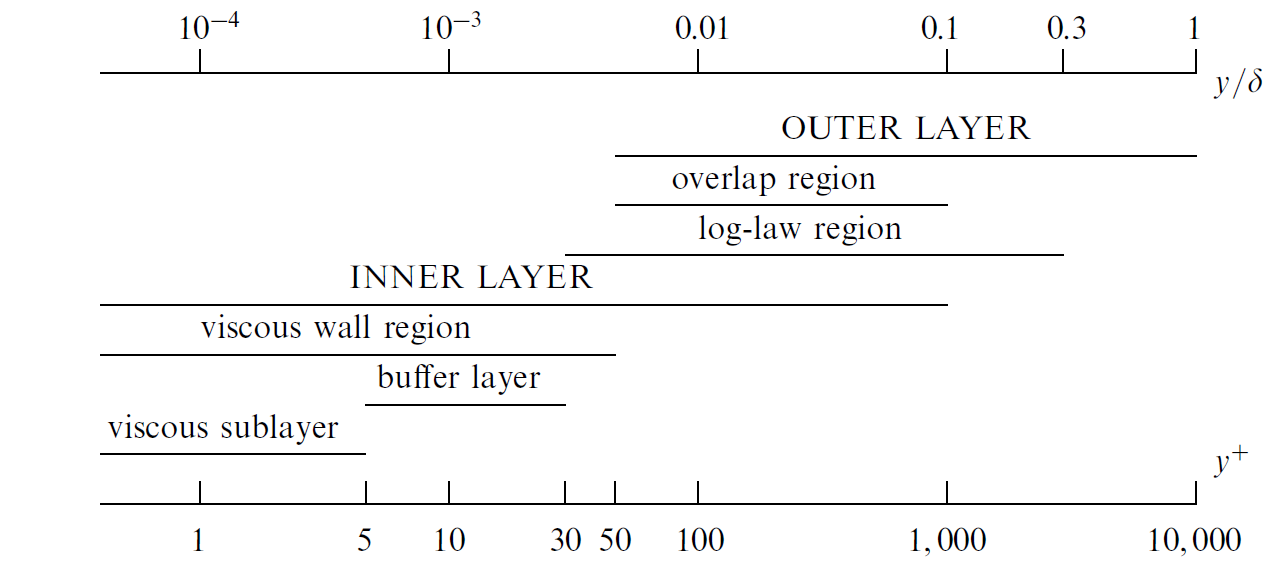
\includegraphics[width=.75\textwidth]{images/wall-regions.png}
  \caption{Depiction of wall regions at different $y^+$ from Pope \cite{popeTurbulentFlows2000}}
  \label{fig:wall-regions}
\end{figure}

There are many excellent tools and methodologies for incompressible turbulent flows that utilize the law of the wall and log law concepts. Ideally, we would want to reuse what has been developed for incompressible turbulence and apply it to compressible turbulence. To do this, an equivalent law of the wall and log law must be derived for compressible turbulence. This is done through a transformation of variables. The historical Van Driest transformation \cite{vandriestTurbulentBoundaryLayer1951} is one such transformation that aimed to achieve this and is still used by researchers to this day. While the Van Driest transformation performs excellently for adiabatic walls, it performs poorly for isothermal walls. The transformation should collapse the compressible velocity profiles onto the incompressible ones. \Cref{fig:vd} demonstrates this concept and how the Van Driest transformation performs for isothermal walls.

\begin{figure}[h]
  \centering
  \vspace{5pt}
  \begin{overpic}[width=.40\textwidth]{images/vdleg1.png}
    \put(35,-5){(a) Adiabatic}
  \end{overpic}
  \quad
  \begin{overpic}[width=.40\textwidth]{images/vdleg2.png}
    \put(35,-5){(b) Isothermal}
  \end{overpic}
  \setlength{\abovecaptionskip}{20pt}
  \caption{\label{fig:vd} Comparison of compressible (colored lines and symbols) to incompressible (solid black) turbulence using Van Driest transformation taken from Trettel \& Larsson \cite{trettelMeanVelocityScaling2016}}
\end{figure}

\subsection{Transformations}
The effects of compressibility on turbulence are typically split into indirect and genuine compressible effects. Indirect effects are due to mean density and temperature variations while genuine effects are caused by dilatational velocity fluctuations and thermodynamic fluctuations. Morkovin \cite{morkovin1962effects} hypothesized that if indirect compressibility effects are properly accounted for, the compressible turbulence distributions should collapse back to their incompressible forms. This hypothesis has been well validated by many experiments and simulations \cite{modestiReynoldsMachNumber2016}. Genuine compressibility effects start to matter at hypersonic (M~$\gtrsim$~5) conditions.

A key feature of compressible flows is that density is no longer constant, that is, $\rho$ and variables that depend on it in the original $y^+$ equation are no longer constant throughout the flow. The famous Van Driest transformation \cite{vandriestTurbulentBoundaryLayer1951} adjusts the velocity gradient, $\frac{du}{dy}$, to match log layer scaling. The transformed velocity then yields a transformed $u^+$. Van Driest chose to evaluate $\rho$ dependent terms at the wall; this yields a transformed $y^+$. The Van Driest transformed wall distance and nondimensional velocity are shown in \Cref{eqn:vd1} and \Cref{eqn:vd2}, where the $u^+$ in \Cref{eqn:vd1} is the untransformed $u^+$ with $u_\tau$ evaluated at the wall.

\begin{align} %van-driest
  U^+_{VD} & = \int^{u^+}_0 \sqrt{\frac{\langle\rho\rangle}{\langle\rho_w\rangle}}du^+ \label{eqn:vd1} \\[0.5ex]
  Y^+_{VD} & = \frac{(u_\tau)_w y}{\nu_w} \label{eqn:vd2}
\end{align}

Trettel \& Larsson formulated an improved compressibility transformation \cite{trettelMeanVelocityScaling2016} by assuming Morkovin's scaling applies everywhere in the flow. Prior researchers made similar transformations based on Morkovin's scaling, but other assumptions were also used, such as the Reynolds stress being zero in the viscous sublayer. Trettel \& Larsson don't use any other assumptions in their transformation derivation. The resulting transformation of $u^+$ and $y^+$ from their stress balance and scaling arguments are displayed in \Cref{eqn:tl1} and \Cref{eqn:tl2}. Compare to \Cref{eqn:vd1} and \Cref{eqn:vd2} and notice that local evaluations of density are used, and a more complicated $u^+$ equation is derived. We will see how much more powerful this transformation is.

\begin{align} %TL
  U^+_{TL} & = \int^{u^+}_0 \sqrt{\frac{\langle\rho\rangle}{\langle\rho_w\rangle}} \left[1 + .5\frac{1}{\langle \rho \rangle} \frac{d \langle \rho \rangle}{dy} y-\frac{1}{\langle \mu \rangle}\frac{d \langle \mu \rangle}{dy}y \right]du^+ \label{eqn:tl1} \\[0.5ex]
  Y^+      & = \frac{u_\tau(y) y}{\nu(y)} \label{eqn:tl2}
\end{align} % include first section

\newpage
\section{Analysis \& Comparisons}
\subsection{Simulation Overview \& Governing Equations}

The governing equations for the DNS of compressible turbulent channel flows are:

\begin{align}
  %NS DNS eqns
  \frac{\partial \rho}{\partial t}+\frac{\partial (\rho u_i)}{\partial x_i}           & = 0                                                                                                           \\[.5ex] % continuity
  \frac{\partial (\rho u_i)}{\partial t}+\frac{\partial (\rho u_i u_j)}{\partial x_j} & =-\frac{\partial p}{\partial x_i}+\frac{\partial \sigma_{i j}}{\partial x_j}+f \delta_{i 1} x \label{eqn:mom} \\[.5ex] % NS, f term is forcing function to enforce mom conservation
  \frac{\partial (\rho E)}{\partial t}+\frac{\partial (\rho u_j H)}{\partial x_j}     & =-\frac{\partial q_j}{\partial x_j}+\frac{\partial (\sigma_{i j} u_i)}{\partial x_j}+f u_1 \label{eqn:eng}    % energy, f here is for enforcing energy conservation
\end{align}

Where the $f$ terms in \Cref{eqn:mom} and \Cref{eqn:eng} serve to enforce a constant mass flow rate in time and $\delta_{ij}$ is the Kronecker delta \cite{modestiReynoldsMachNumber2016}. The stress tensor and thermodynamic variables are defined as:

\begin{align}
  \sigma_{i j} & =\mu\left(\frac{\partial u_i}{\partial x_j}+\frac{\partial u_j}{\partial x_i}-\frac{2}{3} \frac{\partial u_k}{\partial x_k} \delta_{i j}\right) \\[.5ex] %stress tensor
  q_j          & =-k \frac{\partial T}{\partial x_j}                                                                                                             \\[.5ex] %heat
  E            & =c_v T+u_i u_i / 2                                                                                                                              \\[.5ex] %energy E
  H            & =E+p / \rho                                                                                                                                     %enthalpy
\end{align}

For an idea on how expensive DNS is, Pope states that the explicit timestep is roughly on the order of 10\% of the Kolmogorov time scale and the minimum grid spacing is of the order of the Kolmogorov length scale. If we relate this to results we have seen in class, we get a simplistic but informative estimation of the DNS cost.

\begin{align*} %dns grid
  \Delta x & \sim  2.5 \ \eta,  \ \eta \sim Re^{-3/4}         \\
  \Delta t & \sim  .1 \ \tau_\eta, \ \tau_\eta \sim Re^{-1/2}
\end{align*}

\subsection{Transformation Results}
In this section the compressible and incompressible DNS results for the four different transformations studied by Modesti \& Pirozzoli are displayed.
\subsubsection{Velocity Comparison}
The equivalent friction Reynolds number is defined as $Re_{\tau_i} = \frac{\delta(y_i)}{\delta_\nu}$, where $\delta(y_i)$ is the characteristic length scale after applying the y coordinate transformation.  Notice that all cases are for Mach 1.5, except for the bottom right figure in a set, which is at Mach 3. Performance of the transformation is registered as its ability to collapse the compressible turbulence profiles to the incompressible profiles. First, observing the classic Van Driest transformation in \Cref{fig:v-vd}, we see poor performance at all Reynolds numbers (notice $Re_\tau$ and $Re_{\tau_D}$ are identical). The compressible velocity profile varies the most at the low Reynolds number case and performance of the transformation is exacerbated by an increase in the Mach number.

\begin{figure}[h]
  \centering
  \setlength{\abovecaptionskip}{20pt}

  \begin{tabular}{
    >{\centering\arraybackslash}m{.30\textwidth}  @{\quad}
    >{\centering\arraybackslash}m{.50\textwidth}
    }
    % Row 1: the two images, each centered in a fixed‐height cell
    
\includegraphics[width=\linewidth]{images/van-driest-mean-table.png}
     &
    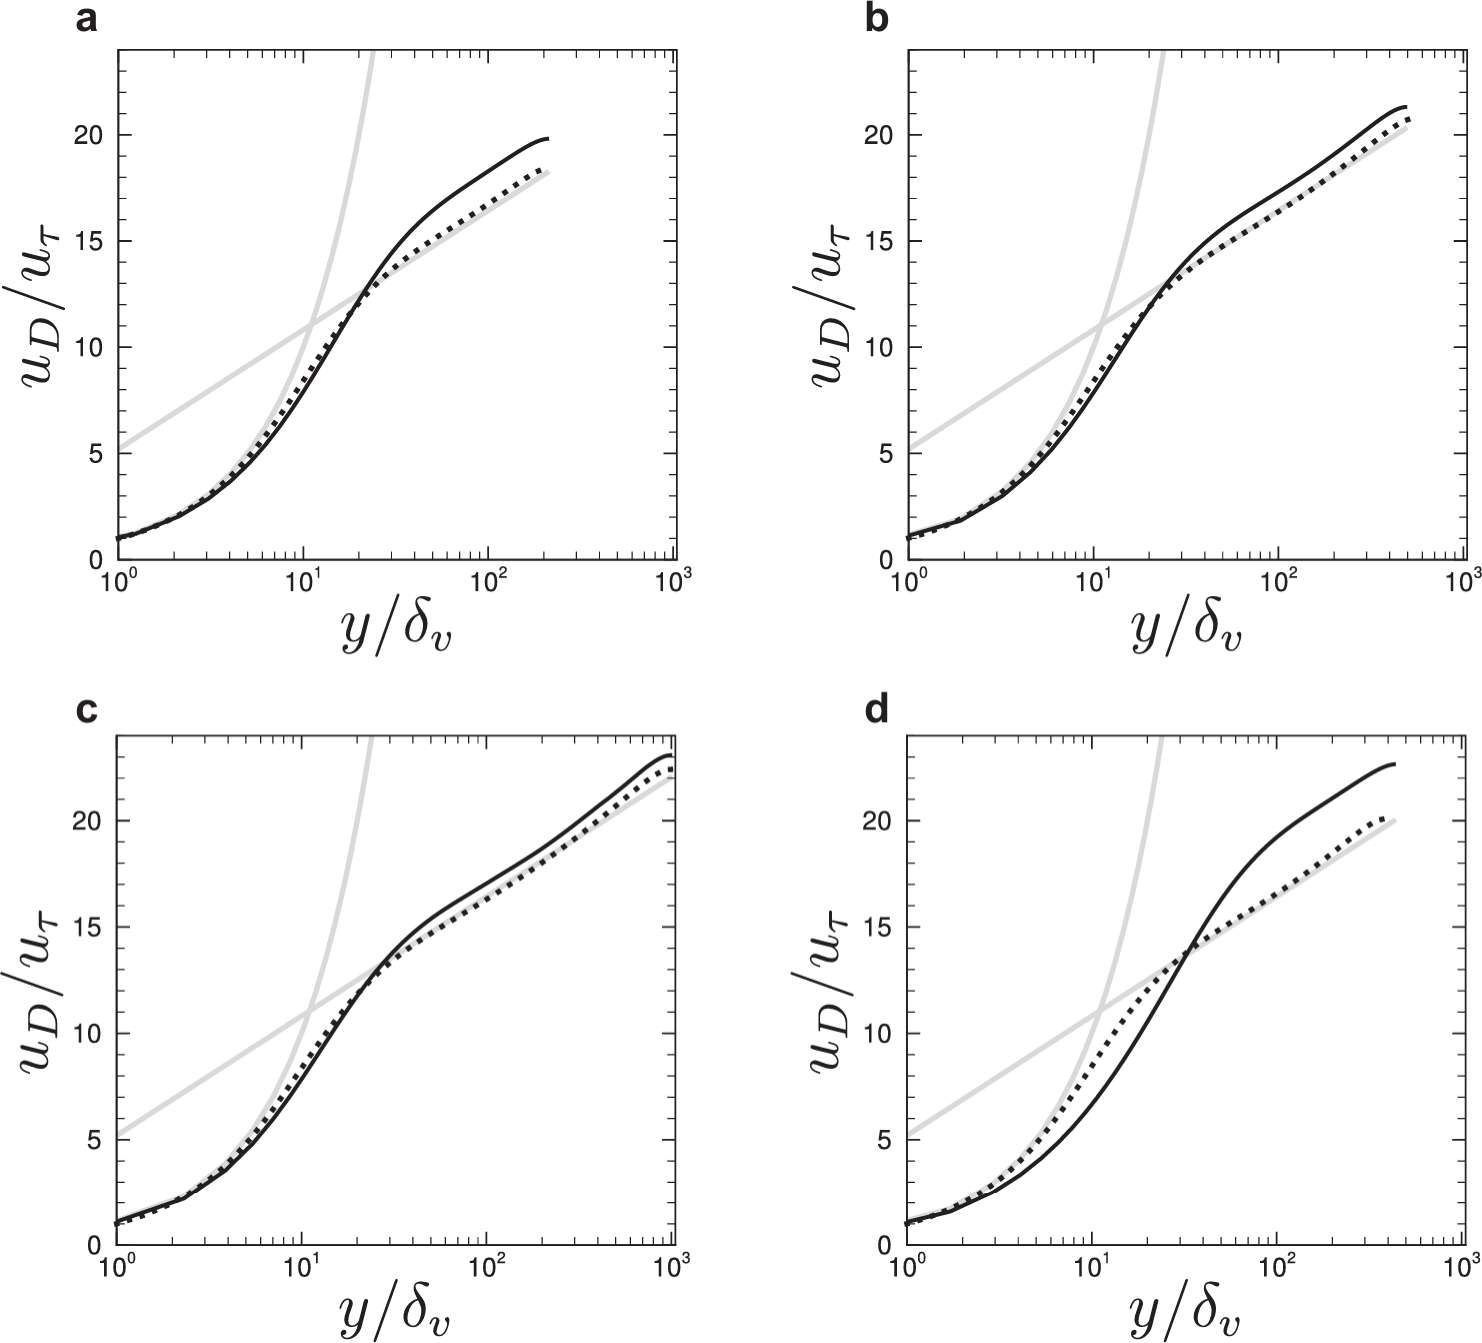
\includegraphics[width=\linewidth]{images/van-driest-incomp-compare1.png}
    \\[1ex]
    % Row 2: the two sub‐captions, same baseline
    (a) Conditions
     &
    (b) Velocity profiles
  \end{tabular}

  \caption{\label{fig:v-vd}
    Velocity comparison of compressible (solid black) to incompressible (black dots) DNS
    using Van Driest transformation taken from Modesti \& Pirozzoli \cite{modestiReynoldsMachNumber2016}}
\end{figure}



\subsubsection{Reynolds Stress Comparison}
Next, the Reynold's stress components are compared for each compressibility transformation. The scaling arguments utilized in the Van Driest, Huang, and Trettel \& Larsson transformations all yield a simple transformation that can be applied to each Reynolds stress component, $\tau_{ij} \Rightarrow \frac{\langle \rho \rangle}{\langle \rho_w \rangle}\tau_{ij}$. Brun's transformation yields a slightly different result for the diagonal components of the Reynolds stress tensor, $\tau_{{ii}_B} = \frac{\langle \rho \rangle}{\langle \rho_w \rangle}(\frac{y}{y_B}\frac{\langle \mu_w \rangle}{\langle \mu \rangle})^2 \tau_{ii}$. The format of the comparisons is the same as the mean velocity transformations. First, Van Driest's transformation is shown in \Cref{fig:r-vd}.

\begin{figure}[ht]
  \centering
  \setlength{\abovecaptionskip}{20pt}

  \begin{tabular}{
    >{\centering\arraybackslash}m{.30\textwidth}  @{\quad}
    >{\centering\arraybackslash}m{.50\textwidth}
    }
    % Row 1: the two images, each centered in a fixed‐height cell
    
\includegraphics[width=\linewidth]{images/van-driest-reynolds-table.png}
     &
    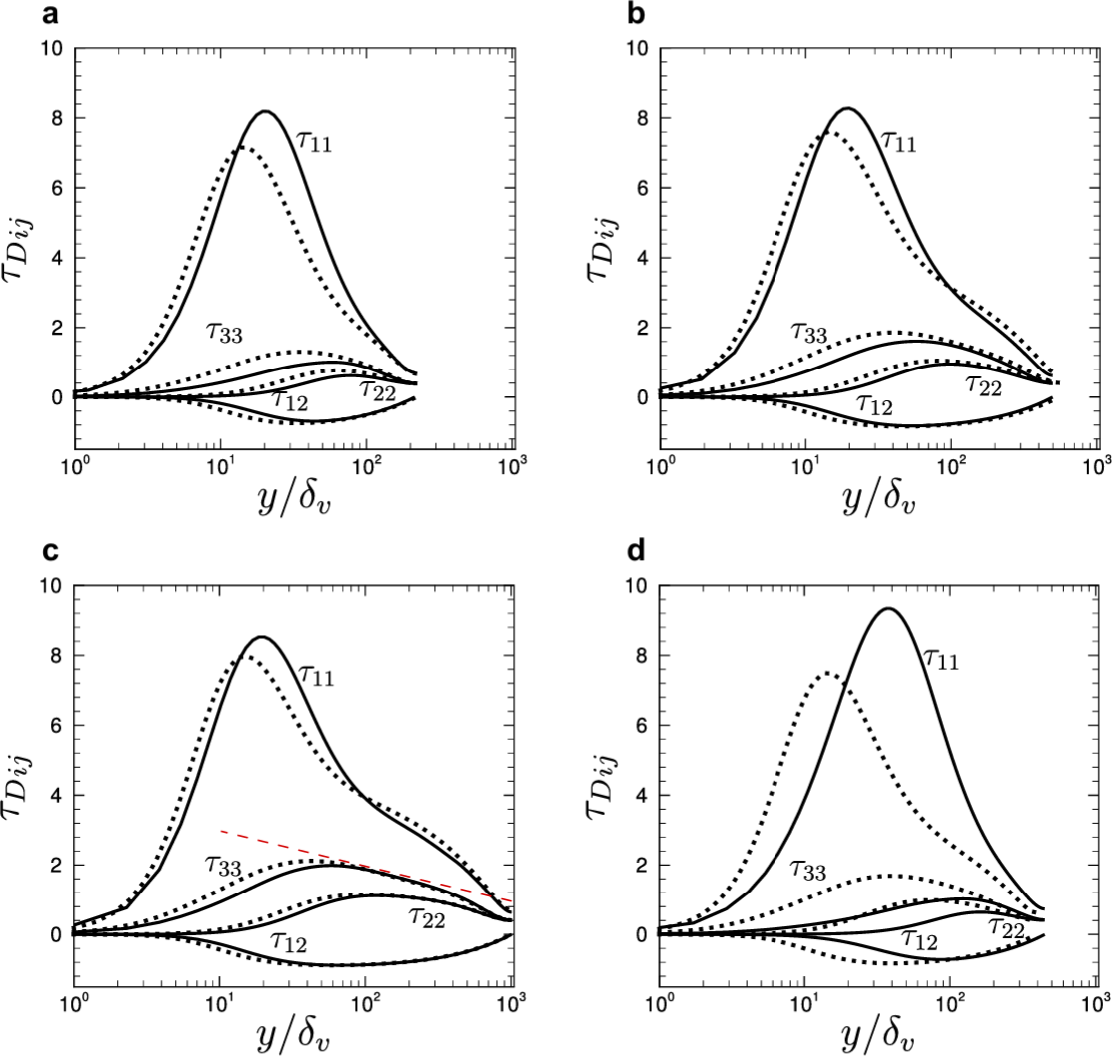
\includegraphics[width=\linewidth]{images/van-driest-incomp-compare2.png}
    \\[1ex]
    % Row 2: the two sub‐captions, same baseline
    (a) Conditions
     &
    (b) Reynolds stress profiles
  \end{tabular}

  \caption{\label{fig:r-vd}
    Reynolds stress comparison of compressible (solid black) to incompressible (black dots) DNS using Van Driest transformation taken from Modesti \& Pirozzoli \cite{modestiReynoldsMachNumber2016}}
\end{figure} % include second section

\newpage
\section{Conclusions}
Four compressibility transformations at varying Mach and Reynolds numbers were presented. The transformation of Trettel \& Larsson showed excellent performance for velocity, collapsing to the incompressible form and demonstrating Mach and Reynolds number independence. Good performance was also observed by Huang/Tretell \& Larsson's transformation for Reynolds stress, with some overshoot at the peak component. Recent studies \cite{hasanIntrinsicCompressibilityEffects2025} have demonstrated that the peak value overshoot is due to the outward shift in the turbulent and viscous shear stresses that lead to the production of streamwise turbulent stress. Trettel \& Larsson's transformation is still well utilized in current research and has been cited 315 times to date since its publication in 2016. More research is needed to investigate turbulence and related transformations at high Mach numbers, where genuine compressibility effects start to matter. % include third section

\clearpage % bibliography section printed, start first page with plain style
\thispagestyle{plain}
\begin{singlespace} % bib should be single spaced
  %\printbibliography[title={Bibliography},heading=bibintoc] % prints bib and adds to toc for biber
  \renewcommand{\refname}{Bibliography} % names bibliography for artilce document when using biber instead of setting it equal to file name
  %\renewcommand{\bibname}{Bibliography} same but for report or book class
  \bibliographystyle{new-aiaa}  % or another BibTeX .bst file you want to use
  \bibliography{references.bib}     % references.bib must exist in your directory
\end{singlespace}

\end{document}